%%% LaTeX Template: Article/Thesis/etc. with colored headings and special fonts
%%%
%%% Source: http://www.howtotex.com/
%%% Feel free to distribute this template, but please keep to referal to http://www.howtotex.com/ here.
%%% February 2011
%%%
%%% Last updated September 2018 by CDM

%%%  Preamble
\documentclass[11pt,letterpaper]{article}
\usepackage[margin=1.0in]{geometry}
\usepackage[T1]{fontenc}
\usepackage[bitstream-charter]{mathdesign}
\usepackage[latin1]{inputenc}					
\usepackage{amsmath}						
\usepackage{xcolor}
\usepackage{cite}
\usepackage{hyphenat}
\usepackage{graphicx}
\usepackage{float}
\usepackage{subfigure}
\usepackage{sectsty}
\usepackage[compact]{titlesec} 
\usepackage[tablegrid]{vhistory}
\allsectionsfont{\color{accentcolor}\scshape\selectfont}

%%% Definitions
\definecolor{accentcolor}{rgb}{0.0,0.0,0.5} 
\newcommand{\teamname}{Team 10}
\newcommand{\productname}{MedTech}
\newcommand{\coursename}{CSE 4316: Senior Design I}
\newcommand{\semester}{Fall 2020}
\newcommand{\docname}{Project Charter}
\newcommand{\department}{Department of Computer Science \& Engineering}
\newcommand{\university}{The University of Texas at Arlington}
\newcommand{\authors}{Maxwell Pham\\Nikita Menon\\Hemantha Govindu\\Nisarg Shah}

%%% Headers and footers
\usepackage{fancyhdr}
	\pagestyle{fancy}						% Enabling the custom headers/footers
\usepackage{lastpage}	
	% Header (empty)
	\lhead{}
	\chead{}
	\rhead{}
	% Footer
	\lfoot{\footnotesize \teamname \ - \semester}
	\cfoot{}
	\rfoot{\footnotesize page \thepage\ of \pageref{LastPage}}	% "Page 1 of 2"
	\renewcommand{\headrulewidth}{0.0pt}
	\renewcommand{\footrulewidth}{0.4pt}

%%% Change the abstract environment
\usepackage[runin]{abstract}			% runin option for a run-in title
%\setlength\absleftindent{30pt}			% left margin
%\setlength\absrightindent{30pt}		% right margin
\abslabeldelim{\quad}	
\setlength{\abstitleskip}{-10pt}
\renewcommand{\abstractname}{}
\renewcommand{\abstracttextfont}{\color{accentcolor} \small \slshape}	% slanted text

%%% Start of the document
\begin{document}

%%% Cover sheet
{\centering \huge \color{accentcolor} \sc \textbf{\department \\ \university} \par}
\vspace{1 in}
{\centering \huge \color{accentcolor} \sc \textbf{\docname \\ \coursename \\ \semester} \par}
\vspace{0.5 in}
\begin{figure}[h!]
	\centering
   	
\includegraphics[width=0.40\textwidth]{images/Apollo.jpg}
\end{figure}
\vspace{0.5 in}
{\centering \huge \color{accentcolor} \sc \textbf{\teamname \\ \productname} \par}
\vspace{0.5 in}
{\centering \large \sc \textbf{\authors} \par}
\newpage


%\vspace{1 in}
%\centerline{January 13th, 2012}
%\newpage

%%% Revision History
\begin{versionhistory}
  	\vhEntry{0.1}{9.29.2020}{MP|NM|HG|NS}{document creation}
  	\vhEntry{0.2}{9.30.2020}{MP}{Added Risks, Constraints}
  	\vhEntry{0.3}{10.01.2020}{NS}{Added documentation}
  	\vhEntry{0.4}{10.03.2020}{MP|NM|HG|NS}{Complete Draft}
  	 requests}
\end{versionhistory}
\newpage

%%% Table of contents
\tableofcontents
\newpage

%%% List of figures and tables (optional)
\listoffigures
%\listoftables
\newpage
\setcounter{table}{0}

%%% Executive summary sections
\section{Problem Statement}
In the medical field, many professionals use Epic EHR as the main software to store and manage data from patients, medicine, and more. The main issue is that it is not user friendly and has a complex user interface where the user can get lost easily, looking at plenty of menus but nothing of use in a bloated interface. The purpose of the project is to simplify the complexities into a user friendly form so that disorganization is kept at a minimum.
\section{Methodology}
To minimize costs and time, we will be using OpenEMR working as the back end of our project. OpenEMR is an open source software that features electronic medical records, management for medical practices, scheduling, and electronic billing. We are going to build a front-end user interface that will organize the components of OpenEMR that simplifies the workflow and minimizing its usage.
One issue noted is that there is no search engine to find all the user interface elements of Epic EMR, such as dates of patient visits, schedules, amounts of medicine administered, and much more. Each of these components have a keyword to them that can be searched. Another issue is that Epic EHR does not have a streamlined process to billing.
\section{Value Proposition}
The Value Proposition explains how the sponsors will benefit from your work, and why they should invest funding, time, and expertise in supporting your team. Here, you are essentially making a case for the project. There are many ways in which value can be returned to your stakeholders (industrial sponsors, instructors, the university, etc.), list any that may help you convince them to "buy in".
\section{Development Milestones}
This list of core project milestones should include all major documents, demonstration of major project features, and associated deadlines. Any date that has not yet been officially scheduled at the time of preparing this document may be listed by month.
\\
\\
Provide a list of milestones and completion dates in the following format:
\begin{itemize}
  \item Project Charter first draft - Month Year
  \item System Requirements Specification - Month Year
  \item Architectural Design Specification - Month Year
  \item Demonstration of <feature or implementation milestone> - Month Year
  \item Detailed Design Specification - Month Year
  \item Demonstration of <feature or implementation milestone> - Month Year
  \item Demonstration of <feature or implementation milestone> - Month Year
  \item CoE Innovation Day poster presentation - Month Year
  \item Demonstration of <feature or implementation milestone> - Month Year
  \item Demonstration of <feature or implementation milestone> - Month Year
  \item Demonstration of <feature or implementation milestone> - Month Year
  \item Final Project Demonstration - Month Year
\end{itemize}
\newpage

%%% Remaining project charter sections
\section{Background}
The world has been riding high on a technological wave. It has entered every aspect of our life and also has influenced several life threatening procedures as well. We live in a fast paced world where everything is digitized. From spending hours in the local library to researching, we now have access to several pages of target data in just a click.  This has helped us save a lot of time and focus on the vital tasks at hand. 

One such industry that is highly time sensitive is the healthcare industry. Taking down vitals on an hourly patients seems like a mundane task. However, even a minute change in dosage or a difference of an hour can drastically effect the patient outcomes. There are several factors that technology could help improve time and efficiency drastically. While talking to several professionals in the health care field, our team realized several factors that shift focus of health care professionals from patient care to administrative tasks that could easily be automated. 

Although a noble field, it is important to realize after all hospitals are also a business and administrative  are equally important to keep the business running. The medical world definitely has its set of jargon which effect medicine and equipment costs that a non-medical professional could perhaps not interpret. Thus it was important to bridge the gap between medicine and accounting so healthcare specialists are focused on medical duties rather than routine administrative tasks. After talking to professionals at different stages of their career, we reviewed other EHR systems and decided to come up with solutions that help accelerate the process of administrative and management tasks in the health care field. 

EMR, Electronic Medical Records, had slow adoption in the US in 2009 \cite{BeldenJ.L.GraysonR.AndBarnes2009}. This was due to the fact that it lacked efficiency and usability of EMRs currently available. This can increase time and costs, hampering productivity. For one specific example, Epic EMR is known to not be user-friendly and requires training. Medical professionals noted that it takes a long time to bill or fill out information, which cuts time for the patient care. Epic EMR also held 54\% of patients in the US in 2015 \cite{Glaze2015}. If the time it takes for a doctor to enter medical records is effectively shortened, he/she would be able to visit more patients and improve health overall. On the business aspect, more patients go through, which means more money is spent either from them or from insurance companies, which adds to the business's profit.

Dr. Shawn Gieser, our sponsor, outlined this inefficiency and selected our team to work on this project. Currently, we do not have a customer, but we are communicating with medical students and medical professionals to aid us in this project.
\section{Related Work}
According to Capterra, a software research group,  30\% of unsatisfied users noted that their EHR software was difficult to use \cite{Reisenwitz2015}. This stems from navigation issues where the user has to actively find what he/she is looking for, looking into menus, tabs, and often for a long period of time. This has been an issue because they lack specialty specific interfaces. Current EHRs attempt to combine multiple professions into one, which can put stress on one profession to navigate through to find relevant information. \cite{Monica2018}

One solution that was considered was data visualization. In a 2017 study from the University of Illinois at Chicago, they were determining if data visualization benefits healthcare since it is a complex field with many specializations. They do not have an explicit solution, since they concluded that data visualization is in its infancy in healthcare. By having the users interact with visualizations, they create new knowledge applicable to them. From their example, a patient's pain score from 1 to 10 could indicate many things. For a physician, additional medicine may be needed. For a nurse, this may register as a failure in pain management. For a physical therapist, this may indicate the pain came from a therapy session. Either all, some, or none could be correct. By visualizing this through glyphs, colors, and shapes, it could portray more information than data values.
\cite{Boyd2017}

In a study published in the Journal of the American Board of Family Medicine, they compared different physician EHR note designs to determine which design is most efficient for physicians. "Cluttered documentation may contribute adversely to physician readers’ cognitive load, inadvertently obscuring high-value information with less valuable information", researchers noted \cite{Monica2017}. They discovered that physicians did not like the traditional SOAP EHR note design, SOAP standing for: Subject, Objective, Assessment, Plan. Simple modifications, such as using colored text and bold fonts or reorganizing Assessment and Plan to the top, could be used to highlight important information. Hiding irrelevant data also avoids overwhelming physicians with clutter.
 \cite{Belden2017}
 
 These studies are explaining high level concepts and there is also the factor of company licenses and privacy, so finding specific solutions that EHR software implemented can be difficult to find. However, the studies will aid us in the design of the user interface.
\section{System Overview}
This section should describe the overall structure of your software system. Think of it as the strategy for how you will build the system. An architectural "layer" is the top-level logical view, or an abstraction, of your design. Layers should be composed of related elements of similar capabilities, and should be highly independent of other layers, but should have very clearly defined interfaces and interactions with other layers. Each layer should be identified individually and should be unique as to its function and purpose within the system. This section should also contain the high-level block diagram of the layers, as shown in the example below, as well as detailed descriptions of the functions of each layer.

\begin{figure}[h!]
	\centering
 	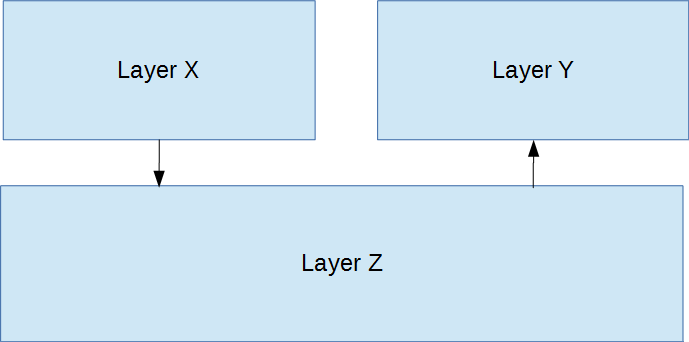
\includegraphics[width=0.60\textwidth]{images/layers}
 \caption{A simple architectural layer diagram}
\end{figure}

\subsection{Layer X Description}
Each layer should be described separately in detail. Descriptions should include the features, functions, critical interfaces and interactions of the layer. The description should clearly define the services that the layer provides. Also include any conventions that your team will use in describing the structure: naming conventions for layers, subsystems, modules, and data flows; interface specifications; how layers and subsystems are defined; etc. 

\subsection{Layer Y Description}
Each layer should be described separately in detail. Descriptions should include the features, functions, critical interfaces and interactions of the layer. The description should clearly define the services that the layer provides. Also include any conventions that your team will use in describing the structure: naming conventions for layers, subsystems, modules, and data flows; interface specifications; how layers and subsystems are defined; etc. 

\subsection{Layer Z Description}
Each layer should be described separately in detail. Descriptions should include the features, functions, critical interfaces and interactions of the layer. The description should clearly define the services that the layer provides. Also include any conventions that your team will use in describing the structure: naming conventions for layers, subsystems, modules, and data flows; interface specifications; how layers and subsystems are defined; etc. 
\section{Roles \& Responsibilities}
The stakeholders in this project will be medical professionals and Dr. Shawn Gieser from the University of Texas at Arlington. Our team consists of four members; Hemantha Govindu, Maxwell Pham, Nikita Menon and Nisarg Shah. For the purpose of this project, we have assigned the roles as follows;

\begin{itemize}
  \item Hemantha Govindu - Scrum master
  \item Maxwell Pham.    - Team Leader
  \item Nikita Menon     - Sponsor contact and Documentation Head
  \item Nisarg Shah      - GitHub manager
\end{itemize}


We intend to keep this roles as they are for the entire duration of the project. We divided this work based on each team members ability and interests. 

Scrum master, Hemantha Govindu, will have the responsibility of maintaining all the scrum-related tasks ranging from deciding who will be assigned what tasks and maintaining the scrum board on Trello, an online scrum-website. 

Our team leader, Maxwell Pham, will have the responsibility of diving all the SRS into sprints and making sure we stay on track for the project deadlines.

Our Documentation Head, Nikita Menon, will be responsible for maintaining all the documentation of code and other tasks and will also be out groups's point of contact to the sponsor, Dr. Gieser.

Out GitHub manager, Nisarg Shah, will be responsible of integrating different features and SRS from branches that other team-members have created into master branch to make sure that the master branch works as planned.
\section{Cost Proposal}
This section contains the approximate budget for the project, where that money will come from, and any other support. This text should be replaced with a discussion and justification of major expenses, but not the actual monetary amounts (that will go in the preliminary budget section below). 

\subsection{Preliminary Budget}
Include a high level budget table for components, fabrication, software licensees, development hardware, etc. This should be in a tabular format broken up into appropriate line items. 

\subsection{Current \& Pending Support}
What are all of the funding sources for the project, and are there any potential funding sources that haven't been secured yet? List all funding sources (including the default funding amount provided by the CSE department) and their dollar amounts.
\section{Facilities \& Equipment}
What lab space, testing grounds, makerspaces, etc. will you need to complete the project? Will you require any specific equipment, and if so, where will you get it (borrow, lease, purchase, outsource, already present in the lab, etc.). This section should occupy 1/2 page.
\section{Assumptions}
An assumption is a belief of what you assume to be true in the future. You make assumptions based on your knowledge, experience or the information available on hand. These are anticipated events or circumstances that are expected to occur during your project's life cycle.

Assumptions are supposed to be true but do not necessarily end up being true. Sometimes they may turn out to be false, which can affect your project significantly. They add risks to the project because they may or may not be true. For example, if you are working on an outdoor unmanned vehicle, are you assuming that testing space will be available when needed? Are you relying on an external team or contractor to provide a certain subsystem on time? If you are working at a customer facility or deploying on their computing infrastructure, are you assuming you will be granted physical access or network credentials?

This section should contain a list of at least 5 of the most critical assumptions related to your project. For example:

The following list contains critical assumptions related to the implementation and testing of the project.

\begin{itemize}
  \item A suitable outdoor testing location will be available by the 3rd sprint cycle
  \item The X sensing system developed by Sensor Consulting Company will be delivered according to specifications by the 4th sprint cycle
  \item Access to the customer installation site will be provided by the 5th sprint cycle
  \item The customer will provide ample power and network connectivity at the installation site
  \item The installation site network infrastructure will allow TCP network traffic on port 8080
\end{itemize}
\section{Constraints}
Constraints are limitations imposed on the project, such as the limitation of cost, schedule, or resources, and you have to work within the boundaries restricted by these constraints. All projects have constraints, which are defined and identified at the beginning of the project.

Constraints are outside of your control. They are imposed upon you by your client, organization, government regulations, availability of resources, etc. Occasionally, identified constraints turn out to be false. This is often beneficial to the development team, since it removes items that could potentially affect progress.

This section should contain a list of at least 5 of the most critical constraints related to your project. For example:

The following list contains key constraints related to the implementation and testing of the project.

\begin{itemize}
  \item Final prototype demonstration must be completed by May 1st, 20XX
  \item The customer will provide no more than two maintenance personnel to assist in on-site installation
  \item Customer installation site will only be accessible by development team during normal business hours
  \item Total development costs must not exceed \$800
  \item All data obtained from customer site must be reviewed and approved for release by the Information Security Office prior to being copied to any internet connected storage medium
\end{itemize}

\section{Risks}
The following high-level risk census contains identified project risks with the highest exposure. Mitigation strategies will be discussed in future planning sessions.

\begin{table}[h]
\resizebox{\textwidth}{!}{
\begin{tabular}{|l|l|l|l|}
\hline
 \textbf{Risk description} & \textbf{Probability} & \textbf{Loss (days)} & \textbf{Exposure (days)} \\ \hline
 Sponsors and Customers (Medical Professionals) meeting delays  & 0.50 & 20 & 10 \\ \hline
 Time Zone conflict for overseas members  & 0.20 & 10 & 5 \\ \hline
 Loss of internet or power while working & 0.05 & 2 & 0.1 \\ \hline
 Loss of code stored locally that is not pushed to repo & 0.1 & 10 & 1 \\ \hline
 Availability of team members staggered due to differing schedules & 0.75 & 5 & 3.75 \\ \hline
\end{tabular}}
\caption{Overview of highest exposure project risks} 
\end{table}
\section{Documentation \& Reporting}
%%% In this section, you will describe all of the various artifacts that you will generate and maintain during the project life cycle. Describe the purpose of each item below, how the content will be generated, where it will be stored, how often it will be updated, etc. Replace the default text for each section with your own description. Reword this paragraph as appropriate.

\subsection{Major Documentation Deliverables}
These deliverables are major grade components of the course. Completing these documents should generally be the sprint goal during the applicable sprint period. Refer to current and previous course syllabi and schedules to estimate the due dates of these items. Remove this explanatory paragraph from your draft, but leave the heading.

\subsubsection{Project Charter}
Describe how this document will be maintained and updated (how often, under what circumstances, etc.). When will the initial version be delivered? When will the final version be delivered?

\subsubsection{System Requirements Specification}
Describe how this document will be maintained and updated (how often, under what circumstances, etc.). When will the initial version be delivered? When will the final version be delivered?

\subsubsection{Architectural Design Specification}
Describe how this document will be maintained and updated (how often, under what circumstances, etc.). When will the initial version be delivered? When will the final version be delivered?

\subsubsection{Detailed Design Specification}
Describe how this document will be maintained and updated (how often, under what circumstances, etc.). When will the initial version be delivered? When will the final version be delivered?

\subsection{Recurring Sprint Items}
The following items will be documented and maintained during each individual sprint. As above, remove this paragraph from your draft, but leave the heading.

\subsubsection{Product Backlog}
How will items be added to the product backlog from the SRS? How will these items be prioritized? Who makes the decision (product owner, group vote, etc.)? What software will be used to maintain and share the product backlog with team members and stakeholders?

\subsubsection{Sprint Planning}
How will each sprint plan be planned? How many sprints will there be (you need to look at the schedules for this course and previous Senior Design II courses during the appropriate semesters to figure this out).

\subsubsection{Sprint Goal}
Who decides the sprint goal? How will you involve your customer in this process?

\subsubsection{Sprint Backlog}
Who decides which product backlog items make their way into the sprint backlog? How will the backlog be maintained (collaboration software, a "scrum board", etc.)?

\subsubsection{Task Breakdown}
How will individual tasks be assigned from the sprint backlog? Will it be up to each team member to voluntarily claim a task, or will it come from the product owner? How will time spent on tasks be documented?

\subsubsection{Sprint Burn Down Charts}
Who will be responsible for generating the burn down charts for each sprint? How will they be able to access the total amount of effort expended by each individual team member? What format will the burn down chart use (include an example burn down chart below).

\begin{figure}[h!]
    \centering
    
\includegraphics[width=0.5\textwidth]{images/test_image}
    \caption{Example sprint burn down chart}
\end{figure}

\subsubsection{Sprint Retrospective}
How will the sprint retrospective be handled as a team? When will this discussion happen after each sprint? What will be documented as a group and as individuals, and when will it be due?

\subsubsection{Individual Status Reports}
What sort of status will be reported by each individual member, and how often will it be reported? What key items will be contained in the report?

\subsubsection{Engineering Notebooks}
How often will the engineering notebook be updated, at a minimum, by each team member? What is the minimum amount of pages that will be completed for each interval, and how long will that interval be? How will the team keep each member accountable? Who will sign of as a "witness" for each ENB page?

\subsection{Closeout Materials}
The following materials, in addition to major documentation deliverables, will be provided to the customer upon project closeout. Remove this paragraph from your draft, but leave the heading.

\subsubsection{System Prototype}
What will be included in the final system prototype? How and when will this be demonstrated? Will there be a Prototype Acceptance Test (PAT) with your customer? Will anything be demonstrated off-site? If so, will there be a Field Acceptance Test (FAT)?

\subsubsection{Project Poster}
What will be included on the poster, what will be the final dimensions, and when will it be delivered?

\subsubsection{Web Page}
What will be included on the project web page? Will it be accessible to the public? When will this be delivered? Will it be updated throughout the project, or just provided at closeout (at a minimum, you need to provide a simple web page at the end).

\subsubsection{Demo Video}
What will be shown in the demo video(s)? Will you include a B-reel footage for future video cuts? Approximately how long will the video(s) be, and what topics will be covered?

\subsubsection{Source Code}
How will your source code be maintained? What version control system will you adopt? Will source code be provided to the customer, or binaries only? If source code is provided, how will it be turned over to the customer? Will the project be open sourced to the general public? If so, what are the license terms (GNU, GPL, MIT, etc.). Where will the license terms be listed (in each source file, in a single readme file, etc.).

\subsubsection{Source Code Documentation}
What documentation standards will be employed? Will you use tools to generate the documentation (Doxygen, Javadocs, etc.). In what format will the final documentation be provided (PDF, browsable HTML, etc.)?

\subsubsection{Hardware Schematics}
Will you be creating printed circuit boards (PCBs) or wiring components together? If so, list each applicable schematic and what sort of data it will contain (PCB layout, wiring diagram, etc.). If your project is purely software, omit this section.

\subsubsection{CAD files}
Will the project involve any mechanical design, such as 3D printed or laser-cut parts? If so, what software will you use to generate the files and what file formats will you provide in your closeout materials (STL, STEP, OBJ, etc.). If your project is purely software, omit this section.

\subsubsection{Installation Scripts}
How will the customer deploy software to new installations? Will you provide installation scripts, install programs, or any other tools to improve the process? Will there be multiple scripts provided (perhaps separate scripts for the graphical front end and back end server software)? 

\subsubsection{User Manual}
Will you customer need a printed or digital user manual? Will they need a setup video? Decide now what will be provided and discuss.

\newpage

%%% References
\bibliographystyle{plain}
\bibliographystyle{reference/IEEEtran_custom}
\bibliography{reference/refs}{}

\end{document}